\documentclass[11pt,a4paper]{article}
\usepackage[margin=2.3cm]{geometry}
\usepackage[T1]{fontenc}
\usepackage{textcomp}
\input{glyphtounicode}
\pdfgentounicode=1
\usepackage{lmodern}
\usepackage{amsmath}
\usepackage{xcolor}
\usepackage{listings}
\usepackage{tcolorbox}
\tcbuselibrary{breakable}
\usepackage{booktabs}
\usepackage{array}
\usepackage{tikz}
\usetikzlibrary{decorations.pathreplacing}
\usepackage{float}
\usepackage{graphicx}
\graphicspath{{images/}}
\usepackage{hyperref}
\hypersetup{colorlinks=true, linkcolor=blue!50!black, citecolor=green!40!black}

\usepackage{accsupp}
% line numbers are drawn but excluded from copied text
\newcommand{\nocopy}[1]{\BeginAccSupp{method=escape,ActualText={}}#1\EndAccSupp{}}
\lstset{
  language=C, basicstyle=\ttfamily\small, keywordstyle={}, commentstyle={}, stringstyle={},
  numbers=left, numberstyle=\footnotesize\nocopy, numbersep=10pt, xleftmargin=2.4em,
  frame=none, columns=fullflexible, keepspaces=true, upquote=true, showstringspaces=false,
  breaklines=true, captionpos=b, aboveskip=1em, belowskip=0.8em
}
\lstdefinestyle{sh}{language=bash, numbers=none, xleftmargin=2.4em}
\renewcommand{\lstlistingname}{Listing}
% code names in the text: grey monospace
\let\origtexttt\texttt
\renewcommand{\texttt}[1]{\textcolor{black!60}{\origtexttt{#1}}}

\newtcolorbox{keyidea}{colback=blue!4, colframe=blue!45!black, title=Key ideas, fonttitle=\bfseries\small}
\newtcolorbox{experiment}{breakable, colback=orange!5, colframe=orange!70!black, title=Experiment, fonttitle=\bfseries\small}
\title{\textbf{OpenMP GPU Memory Access: Coalescing}\\[4pt]\large Lesson 33: neighbouring threads should read neighbouring addresses}
\author{Gustavo Lozano}
\date{November 2026}

\begin{document}
\maketitle

\noindent\textit{\small Source: Deakin \& Mattson~\cite{dm}, Ch.~5 (Using a GPU Effectively),
Sec.~5.2.7 (Memory Coalescence). Prerequisite: \texttt{00-openmp\_target\_teams.pdf} (Lesson 32).}

\section{The idea}
The 32 threads of a warp execute each load \emph{together} (Lesson 32). The GPU memory delivers
data in blocks of 32 bytes, so the hardware merges the 32 addresses of a warp into as few blocks
as possible:
\begin{itemize}
  \item \textbf{Coalesced}: thread $t$ reads element $t$. The 32 doubles (256 bytes) arrive in 8
        blocks, and every byte fetched is used.
  \item \textbf{Not coalesced}: thread $t$ reads element $t\cdot N$. Each thread needs its own
        block: 32 blocks of 32 bytes to use 8 bytes of each, so 3/4 of the traffic is wasted.
\end{itemize}

\begin{figure}[H]
\centering
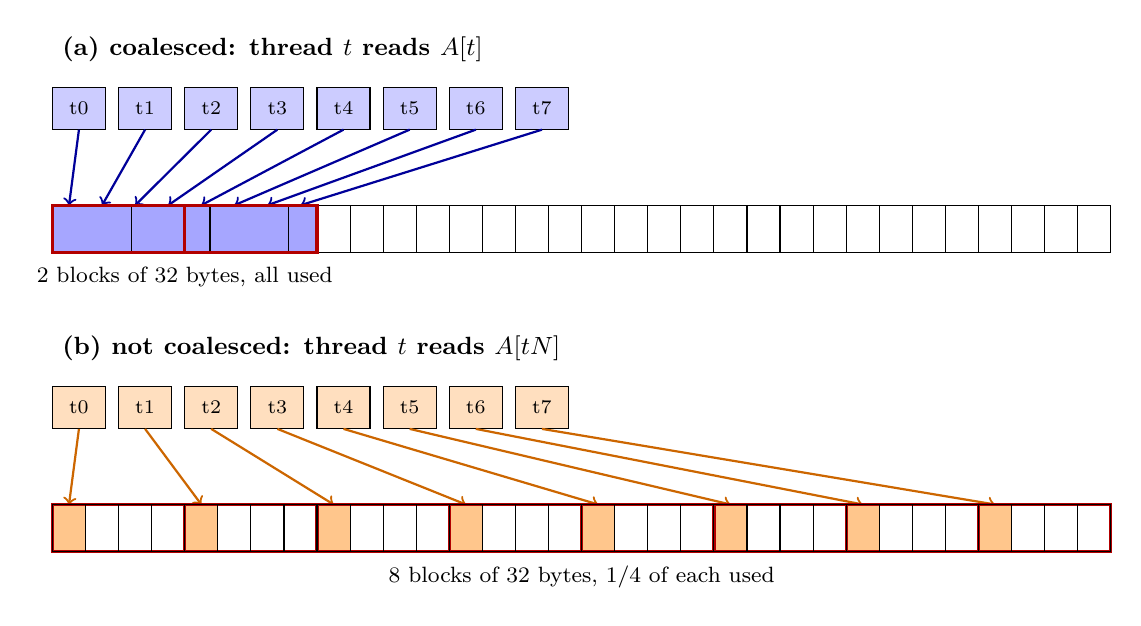
\begin{tikzpicture}[font=\small, x=0.42cm, y=0.6cm]
  \node[anchor=west, font=\small\bfseries] at (0,4.3) {(a) coalesced: thread $t$ reads $A[t]$};
  \foreach \t in {0,...,7} {
    \draw[fill=blue!20] (2*\t,2.6) rectangle ++(1.6,0.9) node[pos=0.5, font=\scriptsize] {t\t};
    \draw[->, thick, blue!60!black] (2*\t+0.8,2.6) -- (\t+0.5,1);
  }
  \foreach \a in {0,...,31} \draw (\a,0) rectangle ++(1,1);
  \fill[blue!35] (0,0) rectangle (8,1); \draw (0,0) grid (8,1);
  \draw[very thick, red!70!black] (0,0) rectangle (4,1); \draw[very thick, red!70!black] (4,0) rectangle (8,1);
  \node[below, font=\footnotesize] at (4,-0.1) {2 blocks of 32 bytes, all used};
  \begin{scope}[yshift=-3.8cm]
  \node[anchor=west, font=\small\bfseries] at (0,4.3) {(b) not coalesced: thread $t$ reads $A[tN]$};
  \foreach \t in {0,...,7} {
    \draw[fill=orange!25] (2*\t,2.6) rectangle ++(1.6,0.9) node[pos=0.5, font=\scriptsize] {t\t};
    \draw[->, thick, orange!80!black] (2*\t+0.8,2.6) -- (4*\t+0.5,1);
    \fill[orange!45] (4*\t,0) rectangle ++(1,1);
    \draw[very thick, red!70!black] (4*\t,0) rectangle ++(4,1);
  }
  \foreach \a in {0,...,31} \draw (\a,0) rectangle ++(1,1);
  \node[below, font=\footnotesize] at (16,-0.1) {8 blocks of 32 bytes, 1/4 of each used};
  \end{scope}
\end{tikzpicture}
\caption{8 threads of a warp loading doubles (small squares) at the same moment. Red frames:
the 32-byte blocks the memory must deliver. (In (b) the elements are $N$ apart; the gap is drawn
shorter.)}
\label{fig:coal}
\end{figure}

\paragraph{CPU vs GPU.} On a CPU each thread runs its own loop, and what matters is that one
thread's \emph{consecutive iterations} read neighbouring addresses (cache lines). On a GPU what
matters is that \emph{neighbouring threads}, at the same moment, read neighbouring addresses.
The same loop can be good for one and bad for the other.

\section{The code}
$A$ is an $N\times N$ matrix stored by rows, \texttt{A[r*N + c]}, with $N = 8192$ (512\,MiB).
Two kernels read all of it (Listing~\ref{lst:coal}):
\begin{itemize}
  \item \texttt{row\_sums\_gpu} (lines 22--32): thread $r$ sums row $r$. At step $k$ threads
        $r$ and $r+1$ read addresses $N$ apart (line 29): not coalesced.
  \item \texttt{col\_sums\_gpu} (lines 34--44): thread $c$ sums column $c$. At step $k$ threads
        $c$ and $c+1$ read neighbouring addresses (line 41): coalesced.
\end{itemize}
The same two loops also run on the CPU. Every sum must be $N$.

\begin{lstlisting}[caption={\textbf{\origtexttt{target\_coalescing.c}} -- row and column sums of a matrix stored by rows, on the GPU and on the CPU.}, label={lst:coal}]
/*
 * target_coalescing.c -- OpenMP Lesson 33: the order of memory accesses on
 * the GPU (coalescing).
 * Source: Deakin & Mattson (2023), Ch. 5 (Using a GPU Effectively),
 *         Sec. 5.2.7 (Memory Coalescence).
 *
 * A is an N x N matrix stored by rows: A[r*N + c].  Two kernels read all of A:
 *   row sums    : thread r sums row r     -> neighbour threads are N apart
 *   column sums : thread c sums column c  -> neighbour threads are adjacent
 * Both run on the GPU and, for comparison, on the CPU.
 *
 * Compile:  clang -O2 -fopenmp --offload-arch=sm_61 \
 *                 -o target_coalescing target_coalescing.c
 * Run:      OMP_TARGET_OFFLOAD=MANDATORY ./target_coalescing [N]
 */

#include <stdio.h>
#include <stdlib.h>
#include <omp.h>

/* ---- GPU ---------------------------------------------------------------- */
static void row_sums_gpu(const double *A, double *s, long N)
{
    #pragma omp target teams distribute parallel for \
            map(present, alloc: A[0:N*N], s[0:N])
    for (long r = 0; r < N; r++) {
        double sum = 0.0;
        for (long k = 0; k < N; k++)
            sum += A[r * N + k];          /* thread r+1 reads N elements further */
        s[r] = sum;
    }
}

static void col_sums_gpu(const double *A, double *s, long N)
{
    #pragma omp target teams distribute parallel for \
            map(present, alloc: A[0:N*N], s[0:N])
    for (long c = 0; c < N; c++) {
        double sum = 0.0;
        for (long k = 0; k < N; k++)
            sum += A[k * N + c];          /* thread c+1 reads the next element */
        s[c] = sum;
    }
}

/* ---- CPU: the same loops ------------------------------------------------ */
static void row_sums_cpu(const double *A, double *s, long N)
{
    #pragma omp parallel for
    for (long r = 0; r < N; r++) {
        double sum = 0.0;
        for (long k = 0; k < N; k++)
            sum += A[r * N + k];
        s[r] = sum;
    }
}

static void col_sums_cpu(const double *A, double *s, long N)
{
    #pragma omp parallel for
    for (long c = 0; c < N; c++) {
        double sum = 0.0;
        for (long k = 0; k < N; k++)
            sum += A[k * N + c];
        s[c] = sum;
    }
}

/* time one kernel; on the GPU copy s back to check it (not timed) */
static void run(const char *name, void (*f)(const double *, double *, long),
                const double *A, double *s, long N, int gpu)
{
    for (long i = 0; i < N; i++) s[i] = 0.0;
    if (gpu) {
        #pragma omp target update to(s[0:N])
    }
    double t = omp_get_wtime();
    f(A, s, N);
    t = omp_get_wtime() - t;
    if (gpu) {
        #pragma omp target update from(s[0:N])
    }
    long bad = 0;
    for (long i = 0; i < N; i++) bad += (s[i] != (double)N);
    printf("%-16s: %8.1f ms  %7.1f GB/s   correct: %s\n",
           name, 1e3 * t, 8.0 * N * N / t / 1e9, bad ? "NO" : "yes");
}

int main(int argc, char **argv)
{
    long N = argc > 1 ? atol(argv[1]) : 8192;        /* 8192^2 doubles = 512 MiB */
    double *A = malloc(N * N * sizeof(double));
    double *s = malloc(N * sizeof(double));
    for (long i = 0; i < N * N; i++) A[i] = 1.0;     /* every sum is N */

    printf("N = %ld: matrix of %.0f MiB, stored by rows\n",
           N, N * N * 8.0 / (1 << 20));

    #pragma omp target enter data map(to: A[0:N*N]) map(alloc: s[0:N])
    row_sums_gpu(A, s, N);                           /* warm-up, not timed */
    run("gpu row sums", row_sums_gpu, A, s, N, 1);
    run("gpu column sums", col_sums_gpu, A, s, N, 1);
    #pragma omp target exit data map(delete: A[0:N*N], s[0:N])

    run("cpu row sums", row_sums_cpu, A, s, N, 0);
    run("cpu column sums", col_sums_cpu, A, s, N, 0);

    free(A); free(s);
    return 0;
}
\end{lstlisting}

\begin{lstlisting}[style=sh]
clang -O2 -fopenmp --offload-arch=sm_61 -o target_coalescing target_coalescing.c
OMP_TARGET_OFFLOAD=MANDATORY ./target_coalescing
\end{lstlisting}

\begin{keyidea}
\begin{itemize}
  \item A warp's 32 loads are served together; contiguous addresses need few memory blocks.
  \item Coalescing rule: the index that changes from one thread to the next should be the index
        that is contiguous in memory.
  \item The good order for the CPU (each thread walks contiguous memory) can be the bad order for
        the GPU, and the other way round.
\end{itemize}
\end{keyidea}

\section{The experiment}
\begin{experiment}
\textbf{Question:} how much does the order of accesses cost on the GPU, and on the CPU?

Run the program:
\begin{lstlisting}[style=sh]
OMP_TARGET_OFFLOAD=MANDATORY ./target_coalescing
\end{lstlisting}

\textbf{What to observe and answer.}
\begin{enumerate}
  \item Which kernel is faster on the GPU? How close is it to the memory bandwidth of Lesson 30?
  \item Which kernel is faster on the CPU? Why is the winner reversed?
  \item The non-coalesced GPU kernel uses only 1/4 of each block it fetches. Is it 4 times
        slower? If it is less, what could reuse the rest of each block?
\end{enumerate}
\end{experiment}

\paragraph{Answers (read after trying).}

\noindent(1)~Column sums: each warp reads 32 neighbouring doubles at every step, so the
bandwidth should come close to the GPU memory bandwidth. Row sums are several times slower.

\noindent(2)~Row sums: each CPU thread walks along its own row, so every 64-byte cache line is
used in full and the prefetcher streams ahead. Column sums jump $N\cdot 8 = 64$\,KiB at every
step, so each step touches a new cache line (and often a new page). The GPU prefers the opposite
order because its threads move in lockstep.

\noindent(3)~Usually less than 4 times. The GPU caches (L1 and a 1\,MB L2) can keep a fetched
block until the same thread reads its next elements at steps $k+1$, $k+2$, $k+3$. With 8192
threads each holding a block, part of them survive; the rest are fetched again.

\paragraph{Next lesson.} To be planned: more GPU core concepts (the \texttt{loop} construct,
asynchronous execution with \texttt{nowait}), or back to the CPU lessons.

\begin{thebibliography}{9}
\bibitem{dm} T.~Deakin and T.~G.~Mattson. \emph{Programming Your GPU with OpenMP: Performance
  Portability for GPUs}. MIT Press, Cambridge, MA, 2023.
\end{thebibliography}
\end{document}
